\documentclass{farlamp}

% latexmk -pvc -pdfxe -bibtex -interaction=nonstopmode -outdir=build tiny-supfail.tex

\addbibresource{references.bib}
\graphicspath{ {./tiny-supfail-pics/} }

\subject{Report}
\title{Training a tiny SupAmp model on easy tasks}
\subtitle{The influence of failure rate on learning curves}
\author{Richard Möhn}
\date{\today}
\addtitledatatopdf

\begin{document}
\maketitle
\tableofcontents

%%%%%%%%%%%%%%%%%%%%%%%%%%%%%%%%%%%%%%%%%%%%%%%%%%%%%%%%%%%%%%%%%%%%%%
\section{Introduction}

(For a project overview and a glossary, see the
\href{https://github.com/rmoehn/farlamp}{home page of the Farlamp repository.})

\textsc{Bluf}: The learning behaviour is as roughly expected. \Xpa\ compensates
for some overseer failures, although not yet enough to be reliable. Mistakes I
made prevent me from drawing further interesting conclusions from the experiment
results so far. \OQsymbol\ and \TODOsymbol\ mark questions and tasks for future
research.

I ran experiments with a tiny SupAmp model on easy tasks. Small data, short
training times and local execution allow for a tight feedback loop with few
moving parts. Thus I could understand and adapt the code, and fix mistakes
quickly.

The drawback is that it doesn't yield many insights. One result, however, was
encouraging: \Xpa\ does learn to be more reliable than its overseer \AmpHp. The
rest of the results fall into two categories: Results confirming my
understanding of the code and learning behaviour. And results made useless by
mistakes and misunderstanding of mine. Although the latter sounds bad, it is
actually useful to have exposed these mistakes before running more expensive
experiments.

In this report I quickly note and discuss the methods, observations and lessons
learned before I move on. ‘Quickly’ also means that you have to content yourself
with screenshots of TensorBoard instead of pretty plots.

% TODO: Mention the striking result and my having made mistakes.

% - To get a feeling for what is going on.
% - And solve problems with the code with a short feedback loop. → Without having
% to deal with big data, long training times and working in the cloud.
% - Ran experiments with a tiny model on easy tasks.
% - Still found results that are useful, because they open questions for further
% research. See \OQ and \TODO markers.
% - Quickly writing the interesting parts up before I move on.
% - Quickly also entails that I use screenshots of TensorBoard instead of nice
% plots.


\subsection{Terms}

% $X$  & The model that is trained on question-answer pairs. \\
% \Xpa & A predictor derived from $X$ by Polyak averaging and used by
% \Amplify{H'}{\Xpa} to answer sub-questions. \\

Questions are answered by \AmpHp. The resulting (question, answer) pairs are
used to train $X$. From $X$ \Term{\Xpa} is derived by Polyak averaging. This is
the same as in \textcite{CSASupAmp}, except that I introduce the symbol \Xpa\ in
order to separate the learner from the assistant. I distinguish them here,
because they are distinguished in the code. From the code also derive the labels
in the diagrams that you will see later. Table \ref{tab:code-symbols} explains
these using the terms and symbols of this report.

\begin{table}
    \label{tab:code-symbols}
    \caption{Explanations of the labels in the diagrams}
    \begin{tabulary}{\textwidth}{>{\ttfamily}lL}
        \firsthline
        \normalfont label in diagrams   & explanation using the terms of this report \\
        \hline
        accuracy/targets        & validation accuracy of \AmpHp \\
        accuracy/teacher        & validation accuracy of \Xpa \\
        accuracy/train          & training accuracy of $X$ \\
        accuracy/validation     & validation accuracy of $X$ \\
        accuracy\_on/<d>/targets & validation accuracy of \AmpHp\ on
                                  questions/answers of depth $d$ \\
        accuracy\_on/<d>/teacher & validation accuracy of \Xpa\ on
                                  questions/answers of depth $d$ \\
        accuracy/asker/q/train  & training accuracy of $H'$ on imitating the
                                  sub-questions that $H$ would ask \\
        accuracy/asker/q/validation & validation accuracy of $H'$ on imitating
                                      the sub-questions that $H$ would ask \\
        accuracy/asker/a/train  & training accuracy of $H'$ on imitating the
                                  root answers that $H$ would give \\
        accuracy/asker/a/validation & validation accuracy of $H'$ on imitating
                                      the root answers that $H$ would give \\
        \lasthline
    \end{tabulary}
\end{table}

The \Term{depth} $d$ of a question is equal to its height plus one. The height
is defined in \Overfail. They have the same definition, just a different
starting point. Henceforth I will use depth instead of height, in order to be
consistent with \textcite{CSASupAmp} and the SupAmp code.

$\Term{N_a} = N + 1$ is the number of answers a learner can give. – Any of the
numbers of the domain plus a symbol for ‘I don't know’.



%%%%%%%%%%%%%%%%%%%%%%%%%%%%%%%%%%%%%%%%%%%%%%%%%%%%%%%%%%%%%%%%%%%%%%
\section{Method}

I ran SupAmp on the permutation powering task from \textcite{CSASupAmp}. The
code was written originally by Paul Christiano, as far as I know, then modified
by William Saunders, then by me. Fifteen trials were run in total, three each
with error probability $p_F = 0, 0.01, 0.1, 0.3, 1.0$ and the following
configuration:

\begin{itemize}
    \item One-layer transformer for both $H'$ and $X$ (if I understand it
        right).
    \item Permutations of four numbers ($N = 4$), up to the seventh power ($2
        \leqq k \leqq 7$).
    \item Train $X$ with 4000 batches à 50 contexts with 4 root questions and
        answers each. After $X$ is done with 4000 batches, also quit the
        training of $H'$, no matter how far it got.
    \item Other hyperparameters as they were when I got the code.
\end{itemize}

% - SupAmp on permutation powering.
% - Tiny model. Means a one-layer transformer for both H' and X, if I understand
% correctly.
% - Permutation of four numbers, power up to seven.
% - Train for 4000 steps, that is 4000 batches à 50 contexts with 4 questions each
% to train X. However many steps the other threads got done in parallel.
% - Then the same with $p_F \in {0.01, 0.1, 0.3, 1.0}$.
% - Each of these three times.


%%%%%%%%%%%%%%%%%%%%%%%%%%%%%%%%%%%%%%%%%%%%%%%%%%%%%%%%%%%%%%%%%%%%%%
\section{Observations and discussion}

In the following screenshots from TensorBoard the smoothing factor is 0.6 unless
otherwise noted.

\subsection{Without failures ($p_F = 0$)}

\includegraphics[width=0.33\textwidth]{pf0-asker-all}
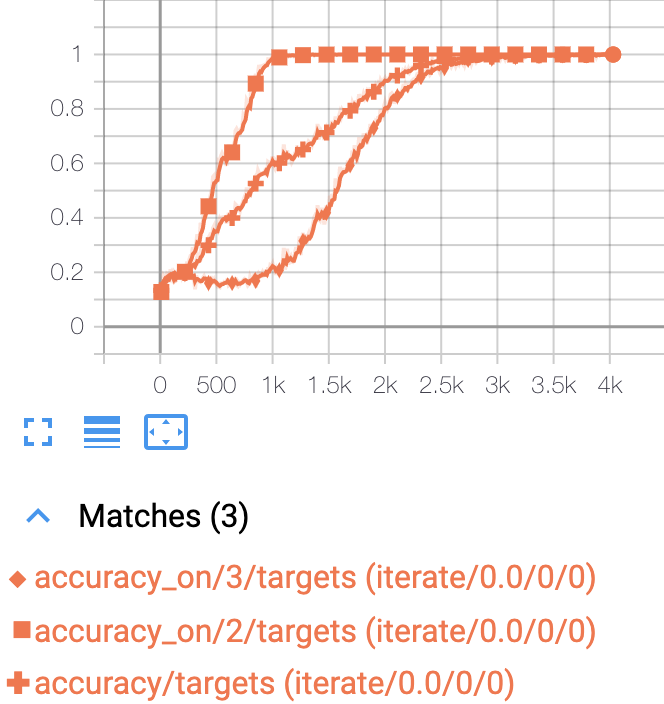
\includegraphics[width=0.33\textwidth]{pf0-targets-all}
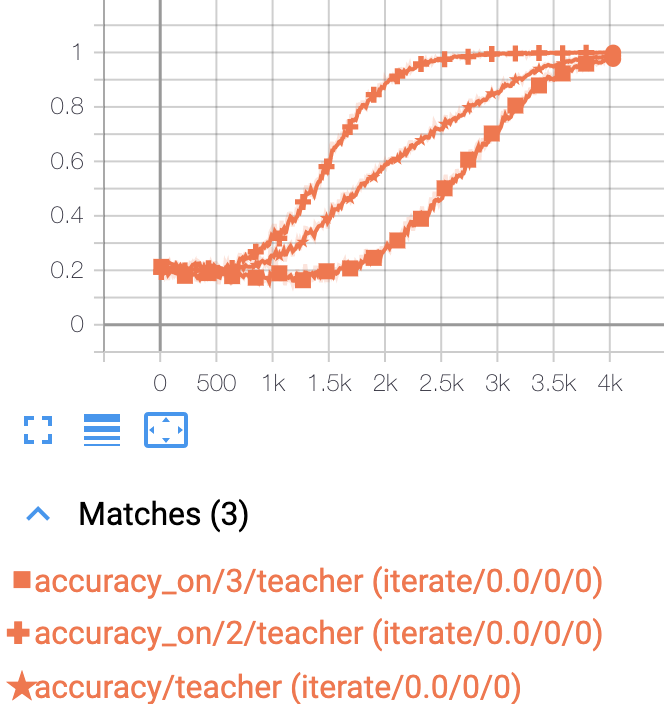
\includegraphics[width=0.33\textwidth]{pf0-teacher-all}

\Obs Given a configuration, the learning curves for all three trials are
similar, the variation between trials is low.
% Include picture of H' and train learning curves for pf = 0 and 0.3.
% When I include pictures, make the names generic, so that I can replace them as
% needed.

\Disc This allows me to select only the first trial of each configuration
for further analysis.

\Obs $H'$ reaches accuracy 1.0 quickest, then \AmpHp\ on depth-2
questions. Thereafter, \AmpHp\ on depth-3 questions and on all questions almost
reach 1.0 together. Finally, \Xpa\ catches up. The accuracy of $X$ lags behind
\AmpHp, and the accuracy of \Xpa\ lags behind that of $X$.

\Disc This is what I roughly expected. These accuracies all depend on each
other. $H'$ needs to become good enough to generate sensible training data for
$X$. At first the only correct answers \AmpHp\ gets are those to depth-1
questions. With the answers to depth-1 questions, \AmpHp\ can answer depth-2
question, which is the next accuracy that goes up. Once depth-2 answers hit the
mark often enough, the training for depth-3 answers becomes effective. Depth-2
and depth-3 answers make up all answers, so the accuracy on all answers is in
between.

\AmpHp\ delivers the training data for $X$ and \Xpa\ is derived from $X$. This
explains the respective lags.

\Obs Training and validation accuracy curves are remarkably close both
for $X$ and $H'$.
% Include pictures of the mentioned accuracies.

\Disc I don't know why this is. \OQ It might be that the validation data
are too similar to the already trained data and therefore not good enough. This
might be because the domains are too small. Or perhaps the learners barely
overfit, because the training data are always random and new.

\Obs The learning curves of \Xpa\ are smoother than those of \AmpHp.
% Include pictures of the mentioned learning curves.
% \begin{picrow}
%     \pic{acc*/targets}
%     \pic{acc*/teacher}
% \end{picrow}

\Disc I guess that this is because of the Polyak averaging. It averages
the weights of the last 1000 steps. This biases the predictions to be similar to
the predictions during the last 1000 steps, and therefore reduces the variance
in the accuracy.

\Obs At the beginning of the training the accuracy of \AmpHp\ and \Xpa\
dips below the initial and expected $\frac{1}{N_a}$. This is subtle, but occurs
in all three runs.
% Include pictures of the appropriate learning curves.

\Disc I don't know why this happens. \OQ It is not important now to find
out.


\subsection{With failures injected ($p_F > 0$)}

Also here the learning curves I will only include the first trial of each
configuration, because the results for the same configuration are almost the
same.

Unfortunately I made two mistakes: I let the training run for too few steps,
stopping it before it converged for depth-3 questions. This means that the
accuracy numbers of \Xpa\ for these are almost useless. And I was confused about
the injecting of errors, putting it in the wrong place or measuring accuracy
wrongly or calculating the theoretical accuracy wrongly. Or all of these
together; I haven't decided how to best resolve the issue. The result is that
the accuracy numbers of \AmpHp\ on depth-3 questions are almost useless as well.

For now I don't have time to clarify my thoughts, fix the code and rerun the
experiments. So I will only note and discuss the few valid observations that are
left.
% See the bottom of the file for what I'd written.

\Obs The accuracy for $p_F = 1.0$ stays at $\frac{1}{N_a}$ for the whole
training.
\Disc This is not surprising. $p_F = 1.0$ means that the training data are
random. With random training data it is impossible to achieve better-than-chance
accuracy. Therefore, I will leave the training curve for this case out of the
discussion.

\Obs The learning curves for all $p_F$, including $p_F = 0$ rise at about the
same time. Only the invisible ceiling that they hit differs.
\Disc This observations appears rather uninteresting. But at least it shows that
in this configuration the injected failures only influence the attainable
accuracy and don't destabilize the training.

\Obs The accuracy of \AmpHp\ on depth-2 questions matches the theoretically
calculated accuracy. The accuracy of \Xpa\ surpasses it in all remaining settings
of $p_F$.

\Disc The former observation is not surprising, since for depth-2 questions $H'$
receives correct inputs (sub-answers to primitve questions) and only its outputs
get laced with randomness. There is nothing between the mechanism that injects
randomness and the accuracy measurement. Therefore the measured accuracy must
match what one would theoretically calculated, given the error injection
mechanism.

The latter observation, however, is striking. (Perhaps the only worthwhile fact
in this report.) \Xpa\ achieves a higher accuracy than \AmpHp, from which its
training data come. This supports my hypothesis that the distillation can
compensate for some of the failures introduced in the amplification.

% I'm not completely sure whether it actually supports the hypothesis, though. –
% When training data contain failures with probability $p_F$.

\Obs With $p_F = 0.01$, the final accuracy of \Xpa\ is 0.9972 (according to
TensorBoard, with the smoothing parameter set to 0.6). This is lower than 0.9997
when $p_F = 0$.

\Disc This speaks against my main hypothesis. – If there was a failure
tolerance, how low can it be? – The reason might be that even the tiny SupAmp
model has too great capacity for this easy task, or, relatedly, that we need
more regularization.

The hypothesis that more regularization leads to a greater failure tolerance,
can be tested. \TODO For example, one could increase the dropout probability
(currently 0.1) and see if the accuracy rises back to $p_F = 0$ levels. Of
course the higher $p_F$, the harder it will be to find a dropout rate that
regularizes away faulty inputs while still allowing learning progress.


%%%%%%%%%%%%%%%%%%%%%%%%%%%%%%%%%%%%%%%%%%%%%%%%%%%%%%%%%%%%%%%%%%%%%%
\section{Points to improve}

\subsection{Length of training}

I noted above that not all learners converged within the 4000 steps that each
trial ran for. In order to ensure convergence and avoid useless results, I could
increase the number of training steps indiscriminately. Better would be to have
the weights saved at the end of training, or even at regular checkpoints. This
will be vital if I move the training to AWS Spot instances, which I'm
considering.


\subsection{Performance}

Much computation is wasted: Measuring code is run frequently, often at every
batch. And a large part of it runs in Python or NumPy space, rather than more
optimized TensorFlow space. $H'$ reaches perfect accuracy within the first 1000
steps ($X$ training steps), but keeps getting trained at full speed. $X$ reaches
perfect accuracy on each successive question depth, yet questions of all depths
continue being sampled uniformly. (The latter might be different when curriculum
learning is turned on.) One should be able to reduce training time by
concentrating ressources where they're needed.


\end{document}

Material collection
-------------------

- What hyperparameters?

- observations
    - low variance between learning curves for same hyperparameters → need to
    look at only one trial per configuration
    - all accuracies approach 1 quickly and without detours
    - behaviour makes sense/almost nothing surprising
        - first H' up to about 0.9, then on/2
        - first on/2 up, then on/3, /targets in between
    - train/validate are rather close

- The teacher learning curves look smoother than the others. This might be
because of Polyak averaging.

- observations with pf = 0

- expected final accuracies at pf = 0.01, 0.1, 0.3, 1.0
    - compared to actual final accuracies
- Why is acc_on/3 less than predicted theoretically?
    - Perhaps not trained to convergence.
- Even with pf = 0.01 the model doesn't get trained to overlook the errors.
    - Small evidence against the main hypothesis. – Would expect that the
    threshold is above 0.01, yet we do get the errors.
    - Might just be that the model has too great capacity/we're not regularizing
    enough.
    → Hypothesis: If I turn up regularization, the accuracies will rise. To a
    point where they don't fall exponentially in the question class/height
    anymore.
    - Of course, at some point the model can't be trained anymore. The error
    probability needs to be low enough that it can be countered with
    regularization weak enough as to not prevent learning.

- → X learns all the mistakes that H' makes

- The acc_on/2/teacher are higher than the acc_on/2/targets.
    - Can't say anything about acc_on/3/*, because training hadn't fully
    converged.
    - Is it because Polyak averaging acts as regularization?

- Training and validation curves are remarkably close.
    - Are the validation data not good enough? Too similar to the already
    trained data?
    - Maybe barely any overfitting, because there are always random new training
    data.

- performance conclusions see case 72
- need to train for longer/add checkpointing

- How do the model errors come about, though? The training data contain randomly
wrong inputs. What does the model learn to do differently when it receives
randomly wrong inputs?


% What I had to throw away, because I made mistakes.

\paragraph{Observation} (When I'm writing about \AmpHp\ and \Xpa, I'm referring
to their final accuracies.) On depth-2 questions \AmpHp\ matches the theoretical
predictions, \Xpa\ surpasses them. On depth-3 questions, both don't reach the
theoretical predictions. Except for one value at $p_F = 0.01$, which I consider
an outlier. Even a failure probability as low as $p_F = 0.01$ prevents the
predictor from reaching perfect accuracy. See table \ref{tab:pred-acc}.

\begin{table}
    \label{tab:pred-acc}
    \caption{Tensorboard smoothing 0.6. In percent.}
    % TODO ideally: Highlight the relevant information.
    \begin{tabular}[.|...|...]
        $p_F$ & $\Pr(a_1 = a_1^\ast)$ & acc. on depth-2 & $\Pr(a_2 = a_2^\ast)$
        & acc. on depth-3 \\
        0.01 & 99.20 & 99.27 & 99.72 & 98.40 & 98.52 & 97.03 \\
        0.10 & 92.00 & 92.31 & 94.50 & 84.80 & 82.02 & 74.28 \\
        0.30 & 76.00 & 75.83 & 78.47 & 59.20 & 51.33 & 37.76 \\
    \end{tabular}
\end{table}


What can I actually say? I made mistakes both in my thinking about what is going
on and in training for too short. It will take some time to fix them. So for now
I can only note that \Xpe reaches a higher accuracy than the training data on
depth-2 questions. (Is this right? Make sure that the ground truth doesn't
contain errors.) (What about $X$? What accuracy does it reach?) This is evidence
for my main hypothesis

% Include pictures of learning curves.

\paragraph{Discussion} Why does \AmpHp\ not match the theoretical predictions on
depth-3 questions? \OQ Did I overlook something in the theoretical calculations?
It might also be because the training hadn't converged yet. I need to train for
longer next time. \TODO

The fact that the learners can't compensate $p_F = 0.01$ is evidence against my
main hypothesis. – If there was a failure tolerance, how low can it be? – The
reason might be that even the tiny SupAmp model has too great capacity for this
easy task, or, relatedly, that we need more regularization. This might explain
why \Xpa\ has greater-than-theoretical accuracy for depth-2 questions. Because of
the Polyak averaging, \Xpa\ acts as an ensemble of neural networks
\parencite{BrowPolyakAvg}. Ensembling is a form of regularization and might
thus compensate for the errors of $H'$.

The hypothesis that more regularization leads to a greater failure tolerance,
can be tested. \TODO For example, one could increase the dropout probability
(currently 0.1) and see if the accuracy rises back to $p_F = 0$ levels. Of
course the higher $p_F$, the harder it will be to find a dropout rate that
regularizes away faulty inputs while still allowing learning progress.

Questions that I can't yet answer: What does $X$/\Xpa\ do differently when
$p_F > 0$? Does it learn to return random answers once in a while like $H'$
does? Or does the noise in the training data just limit learning progress? But
why then does progress stop at exactly the… (Here I noticed that I had made some
mistakes with the failure injection and accuracy measurement.) 
